\documentclass[11pt, oneside]{article}   	% use "amsart" instead of "article" for AMSLaTeX format
\usepackage{geometry}                		% See geometry.pdf to learn the layout options. There are lots.
\geometry{letterpaper}                   		% ... or a4paper or a5paper or ... 
%\geometry{landscape}                		% Activate for for rotated page geometry
%\usepackage[parfill]{parskip}    		% Activate to begin paragraphs with an empty line rather than an indent
\usepackage{graphicx}				% Use pdf, png, jpg, or eps� with pdflatex; use eps in DVI mode
								% TeX will automatically convert eps --> pdf in pdflatex		
\usepackage{amssymb}
\usepackage{amsmath}

\title{Auroux 19, Vector Fields and Line Integrals}
%\author{The Author}
\date{}							% Activate to display a given date or no date

\graphicspath{{/Users/telliott_admin/Dropbox/Tex/png/}}

\usepackage{listings,relsize} 
\lstloadlanguages{R} 
\lstset{language=R,basicstyle=\smaller[1],commentstyle=\rmfamily\smaller, 
  showstringspaces=false,% 
  xleftmargin=4ex,literate={<-}{{$\leftarrow$}}1 {~}{{$\sim$}}1} 
\lstset{escapeinside={(*}{*)}}   % for (*\ref{ }*) inside lstlistings (S code) 

%\section{}
% \subsection*{R code}
% \begin{lstlisting}  \end{lstlisting}
% \begin{center} 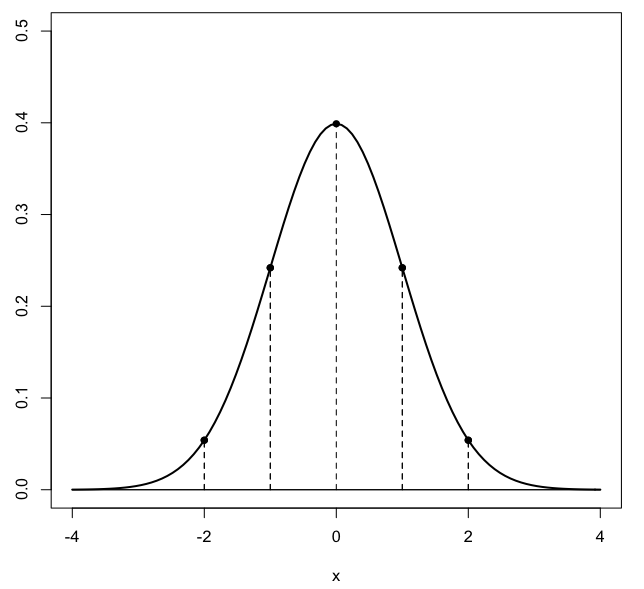
\includegraphics [scale=0.4] {gauss3.png} \end{center}
% \begin{bmatrix} a  &  b \\ c  &  d \end{bmatrix}
% \bigg |_

\begin{document}
\maketitle

\large
\begin{center}
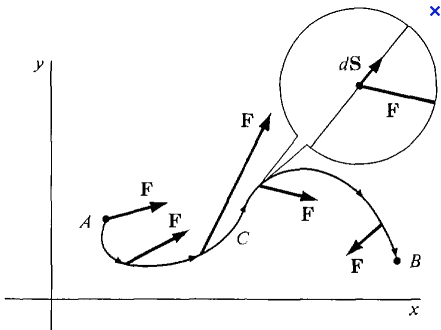
\includegraphics [scale=0.4] {line_integral.png}
\end{center}

Before I start notes on the lecture, I'd like to summarize where we're going.
We imagine an object moving along a trajectory or curve $C$.  It is moving in a vector field $F=f(x,y)$, which varies with position.  At each point along the curve we want to compute $\mathbf{F} \cdot dr$, the dot product of $\mathbf{F}$ with the next little bit of our trajectory.  We take the part of $\mathbf{F}$ in the same direction as $\mathbf{dr}$ and then sum up all those little bits to find the total work
\[ \int \mathbf{F} \cdot \mathbf{dr} = W = \int \mathbf{F} \cdot \mathbf{v} \ dt = \int \mathbf{F} \cdot \mathbf{\hat{T}} \ ds \]
Now, $\mathbf{F} \cdot \mathbf{dr}$ looks a little overwhelming.  How do you integrate a couple of vectors?  Even $\mathbf{F} \cdot \mathbf{v}$ too, for that matter, and what is $\mathbf{\hat{T}}$?  However, if we break this up into components, it will make more sense.

The way to understand $\mathbf{\hat{T}}$ is
\[ \mathbf{dr} = ds \ \mathbf{\hat{T}} \]
What this means is that the vector $\mathbf{dr}$ is in the direction $\mathbf{\hat{T}}$, tangent to the curve, and it has magnitude $ds$, the little bit of arc length.  One way to see this is to divide by $dt$
So 
\[ \frac{\mathbf{dr}}{dt} = \mathbf{v} = \frac{\mathbf{dr}}{ds}  \ \frac{ds}{dt} =  \frac{ds}{dt} \ \mathbf{\hat{T}} =  \left| v \right|\ \mathbf{\hat{T}} \]

So what we are doing here is, at each point along the curve there is the next little change in the $\mathbf{v}$ vector, $\Delta \mathbf{v}$ and we want
\[ \lim_{\Delta \mathbf{v} \to 0} \sum_i \mathbf{F} \cdot \Delta \mathbf{dr} =  \lim_{\Delta t \to 0} \sum_i \mathbf{F} \cdot \frac{\Delta r}{\Delta t} \Delta t= \int_C \mathbf{F} \cdot \mathbf{dr} = \int_{t=t_0}^{t=t_1}  \mathbf{F} \cdot \frac{\mathbf{dr}}{dt} dt \]
Notice the change in limits that goes with the switch to $dt$.
Now, in the end we will actually compute using a formula like this
\[ \int_C \mathbf{F} \cdot \mathbf{dr} = \int <M\hat{i},N\hat{j}> \ \cdot <dx,dy> \]
with one important reservation.  We need to simplify this integral to have a single variable.  We can't really integrate $\int .. \ dx \ dy$.  We can only do this because $x$ and $y$ are related by their trajectory.  We may use a parameter $t$, or perhaps, just express $y$ in terms of $x$.
\[ \int_C \mathbf{F} \cdot \frac{\mathbf{dr}}{dt} \ dt = \int <M,N> \ \cdot <\frac{dx}{dt}, \frac{dy}{dt}> dt \]
\noindent But we have to express things in terms of a single variable.  Then we will have a simple integral over a single variable.
\vspace{ 3 mm}

\noindent Before we do that, let's review a couple of vector fields.
\vspace{ 3 mm}

Field 1.  $F = <i,j>$  This field is the same everywhere $<1,1>$.
\vspace{ 3 mm}

Field 2.  $F = <xi,0>$  This field is proportional to $x$, points left and right ($\Delta y = 0$), and reverses sign at the y-axis.
\vspace{ 3 mm}

Field 3.  $F = <xi,yj>$  This is a radial field, with magnitude proportional to $r$.
\vspace{ 3 mm}

Field 4.  $F = <-yi,xj>$  This is a rotating field.  At $<1,1>$ the field is $<-1,1>$ and $\perp r$.  The magnitude is proportional to $r$, so it's like a rotating disk.
\vspace{ 3 mm}

Example 1.  
\[ F = -yi + xj \]
which is the rotating field.  $r(t)$ is
\[ x = t \]
\[ y = t^2 \]
\[  0 < t < 1 \]
The curve is just $y=x^2$, parametrized.  We have
\[ \int_{t=0}^{t=1} F \cdot \frac{dr}{dt} \ dt = \int_0^1 <-y,x> \ \cdot \ <\frac{dx}{dt},\frac{dy}{dt}> \ dt \]
\[ \ <-t^2, t> \ \cdot <1, 2t> \ dt \]
\[ \int_0^1 t^2 \ dt = \frac{1}{3} \]
We could have said
\[ \int_C  M \ dx + N \ dy = -y \ dx + x \ dy \]
and expressed $y$ in terms of $x$.  This works out the same as before, because $y=x^2$, $dy = 2x dx$ so we have
\[ \int_C  M \ dx + N \ dy = -x^2 \ dx + x \ 2x dx = \frac{1}{3} \]
with limits $x=0$ and $x=1$ (because we had $t=0$ and $t=1$ and $x=t$).
\vspace{ 3 mm}

Example 2.  The curve $C$ is a circle of radius $a$ centered at the origin, going ccw, and the field is $F = <xi,yj>$ .  Now you could set this up and solve it, but you can also notice that
\[ \int \mathbf{F} \cdot \mathbf{\hat{T}} \ ds \]
at every point on the curve the radial vector for the field $<x,y> \perp \mathbf{\hat{T}}$, so the whole thing is is just 0.
\vspace{ 3 mm}

Example 3.  The curve $C$ is again a circle of radius $a$ centered at the origin, going ccw, and the field is the rotating one, $F = <-y,x>$ .  Now you can notice that
\[ \int \mathbf{F} \cdot \mathbf{\hat{T}} =  \left| F \right|\ = \sqrt{x^2 + y^2} = a \]
so this is just
\[ \int_C \mathbf{F} \cdot \mathbf{\hat{T}} ds =  \int_C a \ ds = 2 \pi a^2 \]
if you fail to see this, then you can say we have
\[ \int_C M \ dx + N \ dy = \int_C -y \ dx + y \ dy \]
and 
\[ x = a \ cos\theta, \ \ dx = -a \ sin\theta \ d\theta \]
\[ y = a \ sin\theta, \ \ dy = a \ cos\theta \ d\theta \]
The first term becomes $a^2\ sin^2\theta \ d\theta$ and the second is $a^2\ cos^2\theta \ d\theta$ and so
\[ \int_C a^2 d\theta = 2 \pi a^2 \]



\end{document}  